% !TEX root = ../main.tex


%---------------------------------------------------------------------
% 附录
\clearpage
\ysySection{附录}

\subsection{补充材料}

所有相关材料可以在Github库 \href{https://github.com/TaLEsCuber/CoLabR}{TaLEsCuber/CoLabR} 中找到。

\subsection{实验分工}
\begin{itemize}
	\item 报告撰写：戴鹏辉、杨舒云；
	\item 数据处理：杨舒云、戴鹏辉、黄罗琳；
	\item \textbf{实验过程分工：详见正文；}
	\item 数据记录：丁侯凯、戴鹏辉。
\end{itemize}

\subsection{实验仪器}

\begin{figure}[h!]
	\centering
	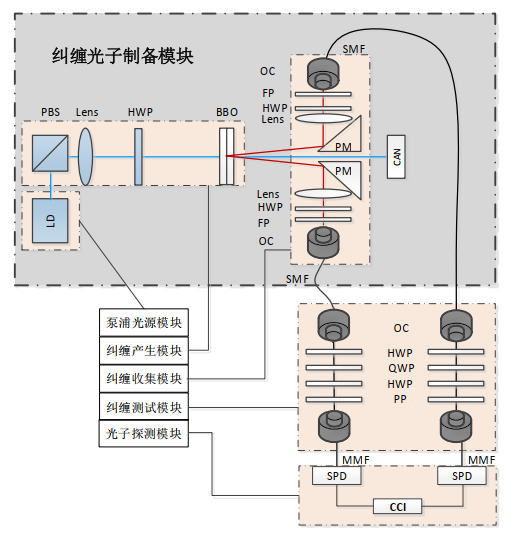
\includegraphics[width=0.6\linewidth]{images/apl2_5_overall_structure_diagram_of_experimental_instrument}
	\caption{实验结构图（各元件简称见讲义）}
	\label{fig:apl25overallstructurediagramofexperimentalinstrument}
\end{figure}


\begin{table}[h!]
	\centering
	\caption{波片角度校准实验用具}
	\begin{tabular}{cccc}
			\hline
			\rowcolor{fgraygreen} \textbf{编号} & \textbf{仪器用具名称} & \textbf{数量} & \textbf{主要参数（型号、规格等）} \\ \hline
			1 & 激光管 & 1 & 波长 808nm \\ 
			2 & 准直架 & 1 & 780nm, $f$=8mm \\ 
			3 & 四轴调整架 & 1 & XY 轴行程: ±2cm，角度调谐范围±4° \\ 
			4 & 偏振分束器 & 2 & 810nm, 偏振消光比$>$1000:1 \\ 
			5 & 偏振片 & 2 & 810nm 增透膜, 消光比$>$500:1 \\ 
			6 & 半波片 & 4 & 810nm 增透膜, 真零级 \\ 
			7 & 1/4 波片 & 2 & 810nm 增透膜, 真零级 \\ 
			8 & 功率计 & 1 & 响应波长: 300-1100nm \\ \hline
	\end{tabular}
\end{table}

\begin{table}[h!]
	\centering
	\caption{纠缠光子测试模块搭建与调节实验用具}
	\begin{tabular}{cccc}
			\hline
			\rowcolor{fgraygreen} \textbf{编号} & \textbf{仪器用具名称} & \textbf{数量} & \textbf{主要参数（型号、规格等）} \\ \hline
			1 & 红光笔 & 1 & 波长 650nm \\ 
			2 & 多模光纤 & 1 & 62.5/125 微米 \\ 
			3 & 准直架 & 2 & 780nm, $f$=8mm \\ 
			4 & 四轴调整架 & 2 & XY 轴行程: ±2cm，角度调谐范围±4° \\ 
			5 & 透镜 & 2 & 直径 25.4cm \\ \hline
	\end{tabular}
\end{table}

\begin{table}[h!]
	\centering
	\caption{Bell 不等式测试及保真度测量实验用具}
	\begin{tabular}{cccc}
			\hline
			\rowcolor{fgraygreen} \textbf{编号} & \textbf{仪器用具名称} & \textbf{数量} & \textbf{主要参数（型号、规格等）} \\ \hline
			1 & 纠缠光子制备模块 & 1 & 泵浦波长: 404.6nm，最大功率 40mW \\ 
			2 & 纠缠源测试模块 & 2 & 波长 810nm \\ 
			3 & 单光子探测器 & 2 & SPCM-AQRH-12 \\ 
			4 & 符合计数仪 & 1 & WT-CC302 \\ 
			5 & 直流电源 & 1 & 0-30V 供电, 三通道 \\ \hline
	\end{tabular}
\end{table}

\clearpage
\subsection{原始数据}
\begin{figure}[h!]
	\centering
	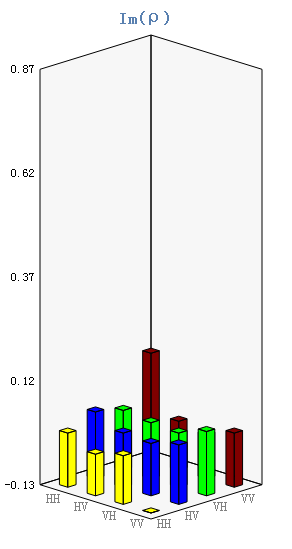
\includegraphics[width=0.7\linewidth]{images/apl2_5_rho_plus_img}
	\caption{密度矩阵虚部}
	\label{fig:apl25rhoplusimg}
\end{figure}

\begin{figure}[h!]
	\centering
	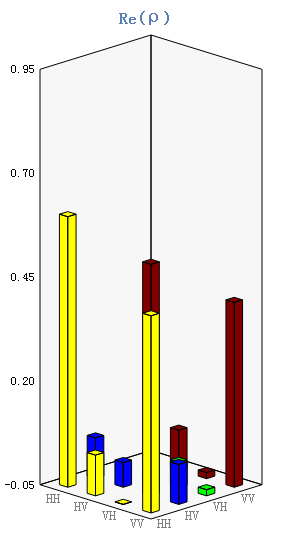
\includegraphics[width=0.7\linewidth]{images/apl2_5_rho_plus_real}
	\caption{密度矩阵实部}
	\label{fig:apl25rhoplusreal}
\end{figure}

\begin{figure}[h!]
	\centering
	\includegraphics[width=0.9\linewidth]{images/E5-OriginalData-1}
	\caption{原始数据1}
	\label{fig:e5-originaldata-1}
\end{figure}

\begin{figure}[h!]
	\centering
	\includegraphics[width=0.9\linewidth]{images/E5-OriginalData-1-old}
	\caption{原始数据1（旧）}
	\label{fig:e5-originaldata-1-old}
\end{figure}

\begin{figure}[h!]
	\centering
	\includegraphics[width=0.9\linewidth]{images/E5-OriginalData-2}
	\caption{原始数据2}
	\label{fig:e5-originaldata-2}
\end{figure}

\begin{figure}[h!]
	\centering
	\includegraphics[width=0.9\linewidth]{images/E5-OriginalData-2-old}
	\caption{原始数据2（旧）}
	\label{fig:e5-originaldata-2-old}
\end{figure}

\begin{figure}[h!]
	\centering
	\includegraphics[width=0.9\linewidth]{images/E5-OriginalData-3}
	\caption{原始数据3}
	\label{fig:e5-originaldata-3}
\end{figure}

\begin{figure}[h!]
	\centering
	\includegraphics[width=0.9\linewidth]{images/E5-OriginalData-4}
	\caption{原始数据4}
	\label{fig:e5-originaldata-4}
\end{figure}

\begin{figure}[h!]
	\centering
	\includegraphics[width=0.9\linewidth]{images/E5-OriginalData-5}
	\caption{原始数据5}
	\label{fig:e5-originaldata-5}
\end{figure}


\clearpage
\subsection{个人签名}
% 专业、年级、姓名、学号、实验名（或编号）和日期
\infoPersonal{物理学强基计划}{2022级}{杨舒云}{22344020}{E5(APL2-5)}{2025年3月28日}

\begin{figure}[htbp]
	\centering
	
\includegraphics[width=0.5\linewidth]{name.png}
	\caption{个人签名：杨舒云}
	\label{fig:name}
\end{figure}

\infoPersonal{物理学强基计划}{2022级}{戴鹏辉}{22344016}{E5(APL2-5)}{2025年3月27日}

\begin{figure}[h!]
	\centering
	\includegraphics[width=0.3\linewidth]{images/name_dph}
	\caption{个人签名：戴鹏辉}
	\label{fig:namedph}
\end{figure}

\infoPersonal{物理学}{2022级}{黄罗琳}{22344001}{E5(APL2-5)}{2025年3月27日}

\begin{figure}[h!]
	\centering
	\includegraphics[width=0.4\linewidth]{images/namw_hll}
	\caption{个人签名：黄罗琳}
	\label{fig:namwhll}
\end{figure}


%---------------------------------------------------------------------
% 参考文献
\clearpage
\ysySection{参考文献}

% 编号、作者、文章名、文章类型、期刊名、发表时间和卷(期):页
\begin{enumerate}[label=\textbf{[\arabic*]},ref=\arabic*]
	\ysyRef{a}{曾谨言}{量子力学卷 I}{M}{第三版. 北京：科学出版社}{2000}{59}  
	
	\ysyRef{b}{牛孝灵}{量子纠缠的制备和应用}{D}{合肥：中国科学技术大学物理系}{2006}{}
	
	\ysyRef{c}{Wikipedia}{Spontaneous parametric down-conversion}{EB}{Wikipedia}{\textit{Accessed March 2025}}{\url{https://en.wikipedia.org/wiki/Spontaneous_parametric_down-conversion}}
	
	\ysyRef{d}{知乎}{BBO晶体的自发参量下转换过程是如何实现的？}{EB}{知乎}{\textit{Accessed March 2025}}{\url{https://www.zhihu.com/question/432445371}}
	
	\ysyRef{e}{CSDN}{量子计算 10 隐变量、贝尔不等式与CHSH}{EB}{CSDN}{\textit{Accessed March 2025}}{\url{https://blog.csdn.net/weixin_42017454/article/details/124145571}}
	
	\ysyRef{1}{Shen, Chao, et al.}{Optimized tomography of continuous variable systems using excitation counting}{J}{Physical Review A}{2016}{94(5): 052327}  
	
	\ysyRef{2}{Řeháček, J., Z. Hradil, and M. Ježek}{Iterative algorithm for reconstruction of entangled states}{J}{Physical Review A}{2001}{63(4): 040303}  
	
	\ysyRef{3}{Řeháček, Jaroslav, et al.}{Diluted maximum-likelihood algorithm for quantum tomography}{J}{Physical Review A}{2007}{75(4): 042108}  
	
	\ysyRef{4}{Shang, Jiangwei, Zhengyun Zhang, and Hui Khoon Ng}{Superfast maximum-likelihood reconstruction for quantum tomography}{J}{Physical Review A}{2017}{95(6): 062336}  
	
	\ysyRef{5}{Ahmed, Shahnawaz, et al.}{Quantum state tomography with conditional generative adversarial networks}{R}{arXiv preprint}{2020}{arXiv:2008.03240}
	
\end{enumerate}